%%%%%%%%%%%%%%%%%%%%%%%%%%%%%%%%%%%%%%%%%%%%%%%%%%%%%%%%%%%%%%%%%%%%%
% LaTeX Template: Project Titlepage Modified (v 0.1) by rcx
%
% Original Source: http://www.howtotex.com
% Date: February 2014
% 
% This is a title page template which be used for articles & reports.
% 
% This is the modified version of the original Latex template from
% aforementioned website.
% 
%%%%%%%%%%%%%%%%%%%%%%%%%%%%%%%%%%%%%%%%%%%%%%%%%%%%%%%%%%%%%%%%%%%%%%

\documentclass[12pt]{report}
\usepackage[a4paper]{geometry}
\usepackage[myheadings]{fullpage}
\usepackage{fancyhdr}
\usepackage{lastpage}
\usepackage{graphicx, wrapfig, subcaption, setspace, booktabs}
\usepackage[T1]{fontenc}
\usepackage[font=small, labelfont=bf]{caption}
\usepackage{fourier}
\usepackage[protrusion=true, expansion=true]{microtype}
\usepackage[english]{babel}
\usepackage{sectsty}
\usepackage{url, lipsum}
\usepackage{tgbonum}
\usepackage{natbib}
\usepackage{hyperref}
\usepackage{xcolor}

\newcommand{\HRule}[1]{\rule{\linewidth}{#1}}
\onehalfspacing
\setcounter{tocdepth}{5}
\setcounter{secnumdepth}{5}



%-------------------------------------------------------------------------------
% HEADER & FOOTER
%-------------------------------------------------------------------------------
%\pagestyle{fancy}
%\fancyhf{}
%\setlength\headheight{15pt}
%\fancyhead[L]{Student ID: 1034511}
%\fancyhead[R]{Anglia Ruskin University}
%\fancyfoot[R]{Page \thepage\ of \pageref{LastPage}}
%-------------------------------------------------------------------------------
% TITLE PAGE
%-------------------------------------------------------------------------------

\begin{document}
{\fontfamily{cmr}\selectfont
\title{ \normalsize \textsc{}
		\\ [2.0cm]
		\HRule{0.5pt} \\
		\LARGE \textbf{\uppercase{ETERNITY: NUMBERS - PI}
		\HRule{2pt} \\ [0.5cm]
		\normalsize July 20, 2019 \vspace*{5\baselineskip}}
		}

\date{}

\author{
		Baiyu Huo 40076004 \\ 
		Concordia University \\
		Department of Computer Engineering }

\maketitle
\tableofcontents
\newpage

%-------------------------------------------------------------------------------
% Section title formatting
\sectionfont{\scshape}
%-------------------------------------------------------------------------------

%-------------------------------------------------------------------------------
% BODY
%-------------------------------------------------------------------------------

\chapter{Description}

	The number PI is a mathematical constant. It used to describe the ratio of the circles' circumference and its diameter, and nowadays it has been used by many formulas in both mathematics and physics. It is an Irrational number which means it can not be present as the ratio of two integers. What's more, PI is also a transcendental number, which means that "it is not the solution of any non-constant polynomial equation with rational coefficients".\citep{wiki:pi} It approximately equals to 3.141592653.
	
	\begin{figure}[h!]
		\centering
		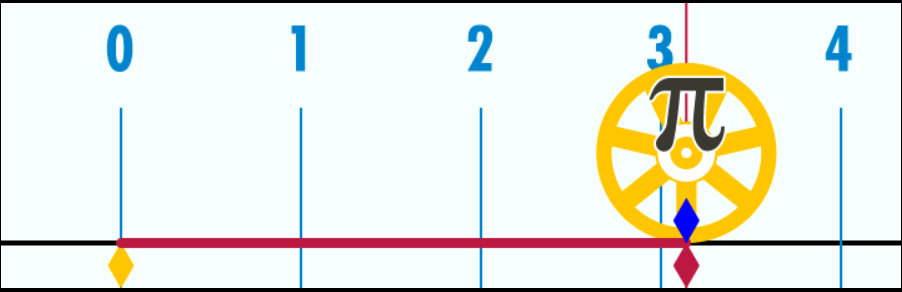
\includegraphics[scale=0.4]{assets/PI.png}
		\caption{PI (Source: Google)}
		\label{fig:universe}
	\end{figure}
	
	
	\section{Difination}
	let C equals circle's circumference, d equals circle's diameter, then PI equals the radio of C and d.
	
	
	\begin{center}
		$PI=\frac{C}{d}$
	\end{center}
	
	\section{Usage} 
	Geometry and trigonometry, Eigenvalues, Inequalities, Fourier transform and Heisenberg uncertainty principle, Gaussian integrals,Projective geometry, Topology etc.
	

\chapter{Interview}
\section{Background}

Dr.Wang is my college teacher, who taught me in Advanced Mathematics, Linear Algebra courses in college. He is a Lecturer of HRBUST (Harbin University of Science and Technology) and Ph.D. student in mathematics, which makes him an ideal candidate for my interviewee.
The interview was made through a video call made from Canada to China on July 5th. 


Interviewee: Yanpeng Wang

Occupation: Lecturer (Mathematics)

Harbin University of Science and Technology

Degree: Doctorate in Mathematics (Ph.D.)


\section{Interview}

- Hi, Dr. Wang, thank you for being my interviewee.  It has been a long time since the last time we met. I know that you've been teaching mathematics for more than 6 years, and currently, you are also a Ph.D. student in mathematics. I currently doing the requirement analysis for a software project which is about the irrational numbers. Can I ask you something about this topic?

- Sure, Let's do it.

\textbf {Q1: How often do you use the calculator?}

A1: As a math teacher, I use the calculator almost on a daily basis. Not only for school works but also in daily life, such as calculating the tax. Sometimes I use a calculator just to make sure that my calculation is right.

\textbf {Q2: Do you think the standard calculator can meet people's computing tasks?}

A2: For most people, I believe, a standard calculator is enough for daily usage.  However, it can not handle the problem domain in some industries such as AI, mathematics, physics, economics, etc. A scientific calculator with special functions is what they need. 

\textbf {Q3: How often do you use PI and in what circumstance you using it?}

A3: I used PI quite often, you know, trigonometric functions highly relies on the angle. To measure the radians, pi is of great importance. In addition to that, pi also appears as a critical spectral parameter in the Fourier transform. Most I prefer to use pi in these problem domains. Generally speaking, in most case, if the problem is related to angle or circle, there will be always a pi in the formula.

\textbf {Q4: It is well known that PI is an irrational number and it’s approximately equal to 3.14 or 22/7. Do you think using 3.14 to replace PI is enough?}


A4: That's a good question.  I hate to say this, but it depends. Usually, in mathematics, we prefer to use pi itself rather than some approximate number. You might think it doesn't have too many difference in using an approximate value, but, in some field such as aerospace, medical etc. It needs to be very precise, so mostly we leave the pi as it is. However, until now we still calculate the pi, but as you know it's an Irrational number, it never gonna end. All in one,  

\textbf {Q5: What accuracy of pi do you think is enough for your usage?} 

A5: I don't like to use the approximate value, but for how much precise its gonna meet our requirement, I guess it's never enough.

\textbf Q6: Could you give us some examples of pi usage in geometry and trigonometry? 

A6: The most well-known usage of pi is to calculate the area of the circle, ring, besides that,  it also be used in Trigonometric function such as sin, cos, tan etc. Just like I said, anything which related to circle or angle, then pi is always the key role.

\textbf{Q7: What do you like or dislike about the calculator?}

A7: What I like about the calculator is that it is really convenient and accurate, except for the complex calculation, for simple arithmetics, it's way faster than human.  However, on the other hand, some of the calculation is hard to perform on a standard calculator. Take trigonometric function as an example, if I want to know how much does "sin pi/5" is, I need to use a special calculator to calculate that, it can not perform in a standard one. And sometimes, to perform a formula in a calculator is also very complex, since most of the calculator doesn't have the brackets. Which means if I want to achieve the brackets priority mechanism, I need to use "record button" to save the value that I calculate in the first place, then reuse them as a part of the second operation. That is really overwhelming.

\textbf{Q8: What function do you think would be an improvement for a calculator?}

A8: If there is some function which will replace the complex operation of a formula would be an improvement, I think. In other words,  if a calculator can save some formula, which can be used anytime would be a really convenient feature. 


\section{Analysis}
According to the interview, the interviewee believes that people in different industry usually has different requirement about the calculator, they are more focusing on some of the special functions that related to his domain. What's more, sometimes the functions in most of the scientific calculators are too general, which might cause a bad user experience, so for some problem domain, a calculator with specific functions is better. In addition, the irrational number pi is widely used in mathematics and physics especially in geometry and trigonometry, such as the angle calculation. For general usage, pi can be used as 3.14, however, in some area, such as research, aerospace and medical, it's better to calculate pi as accurate as possible.


\chapter{Persona}
\section{Yanpeng Wang}
	\begin{figure}[h!]
		\centering
		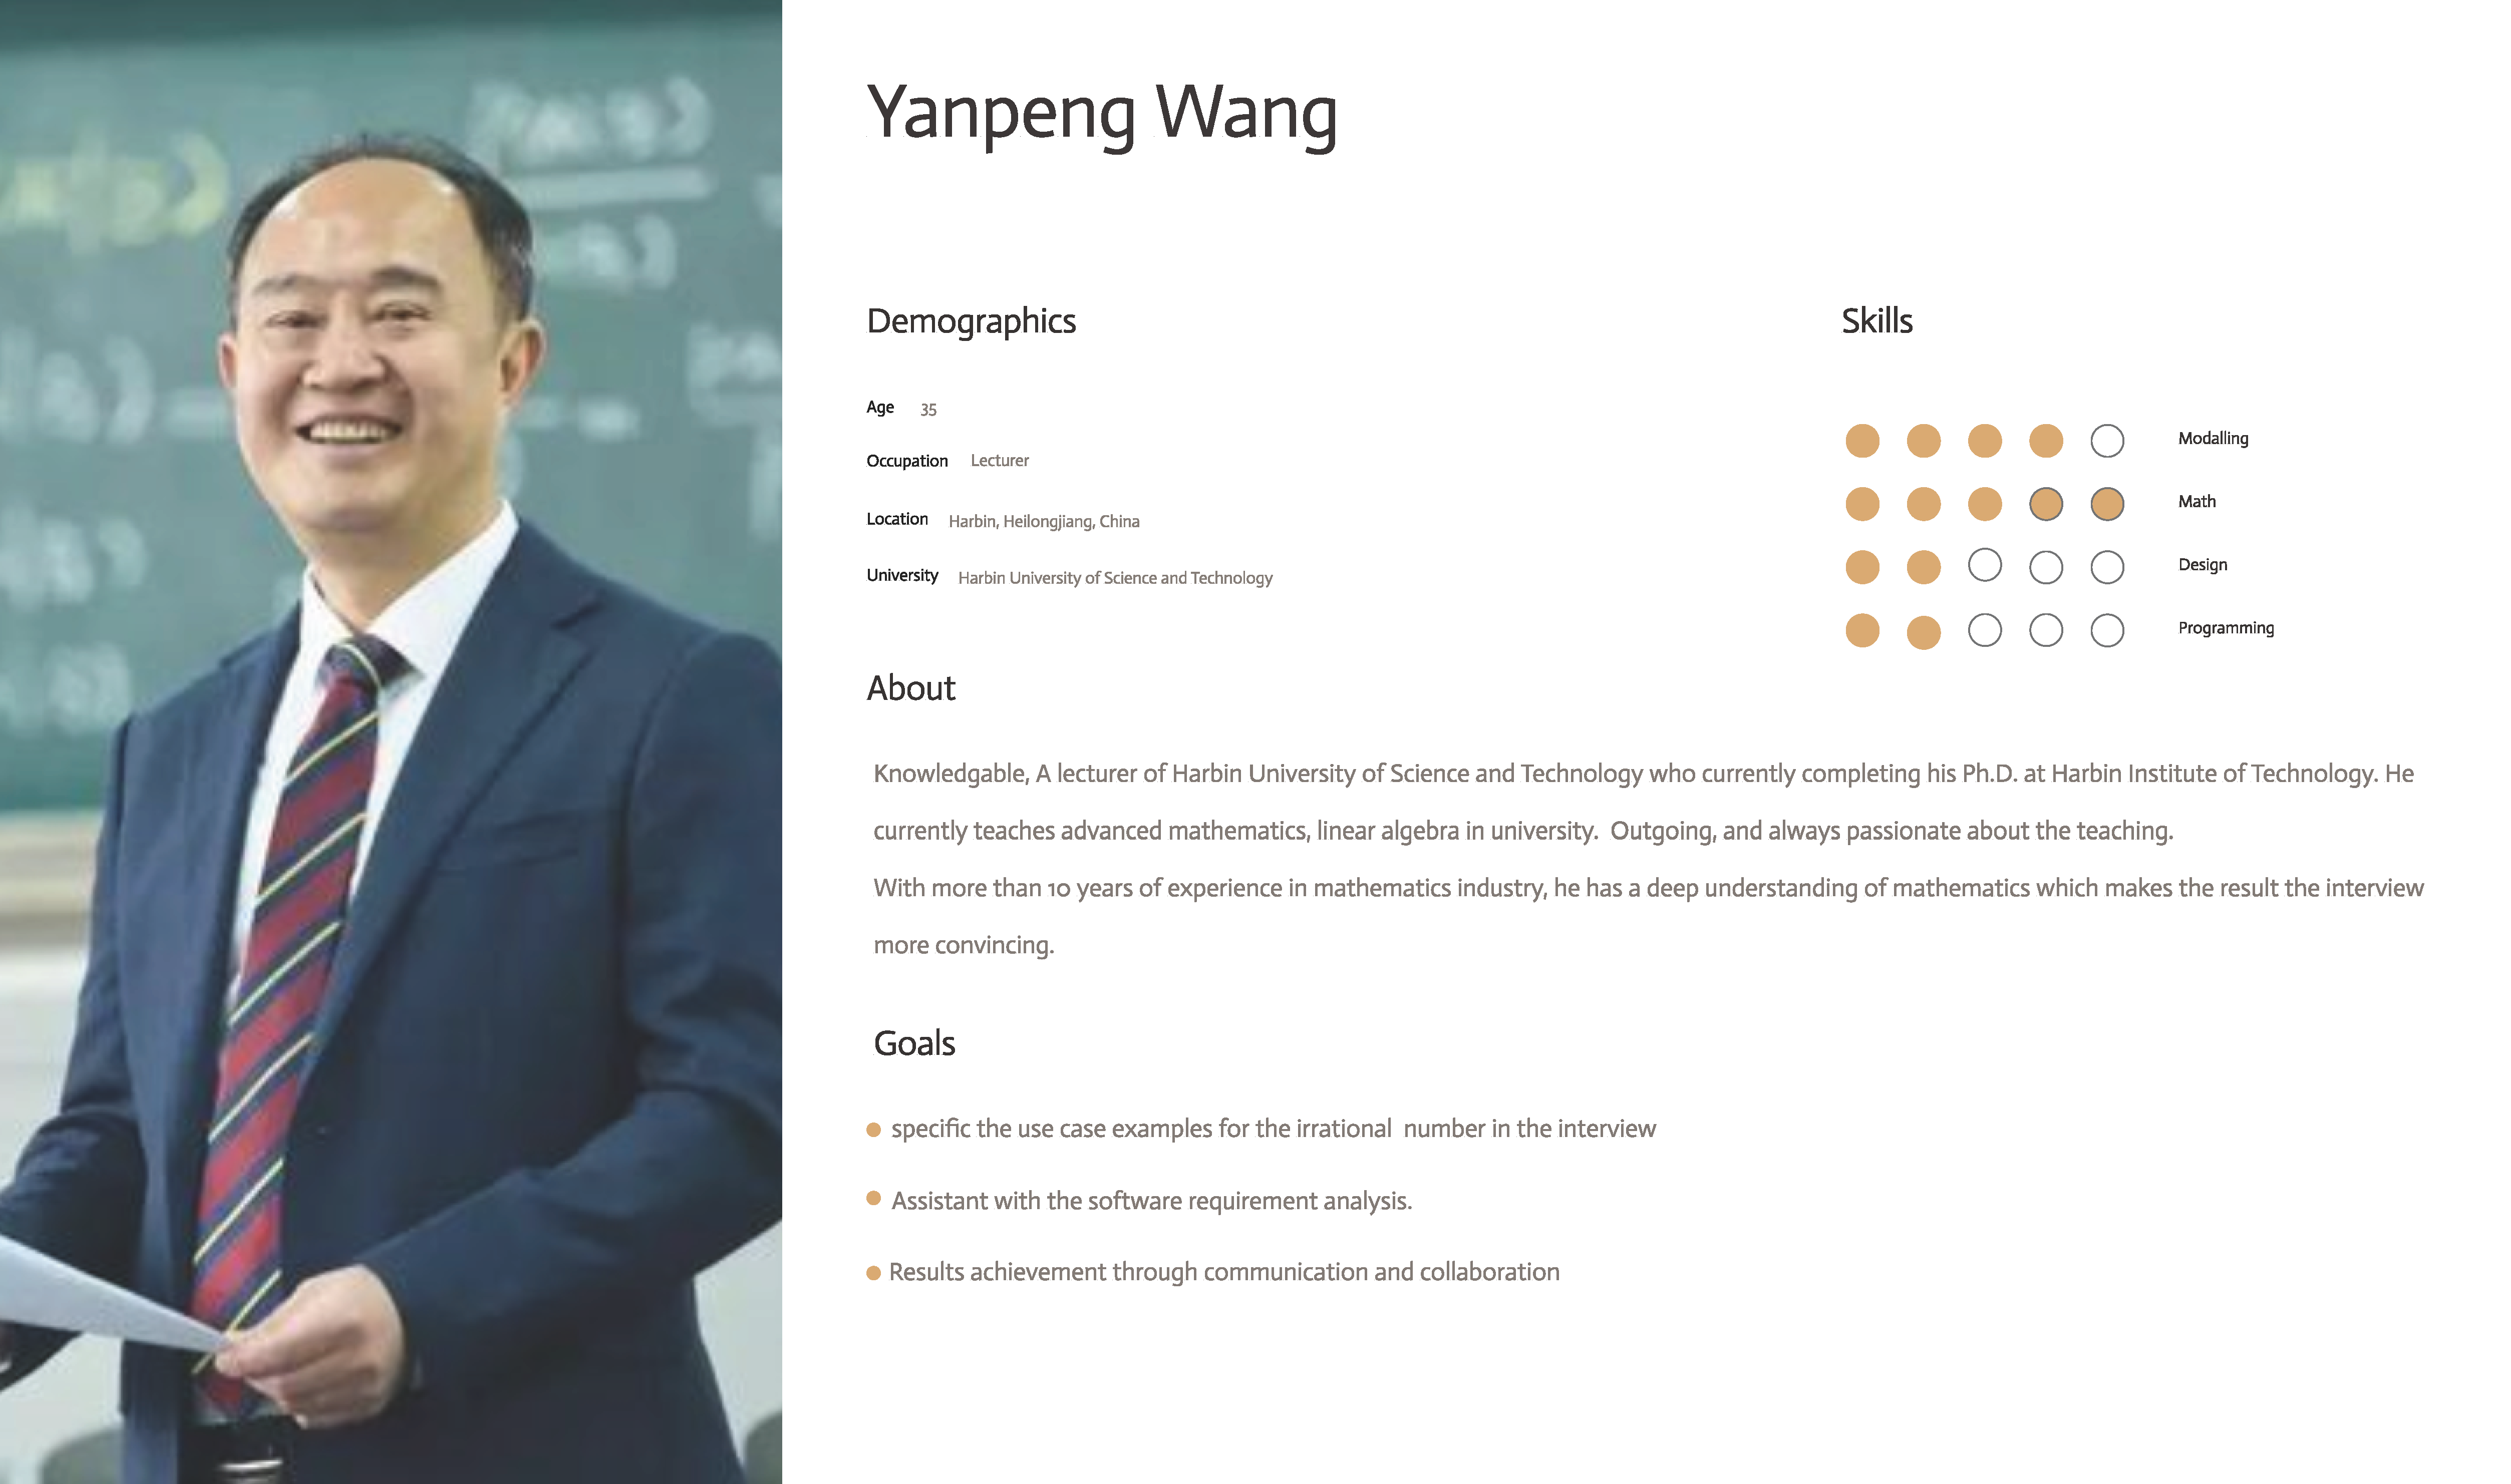
\includegraphics[width=\textwidth]{assets/persona.png}
		\caption{Persona}
		\label{fig:universe}
	\end{figure}

\chapter{Domain Model}
\section{Domain Model Diagram}

	\begin{figure}[h!]
		\centering
		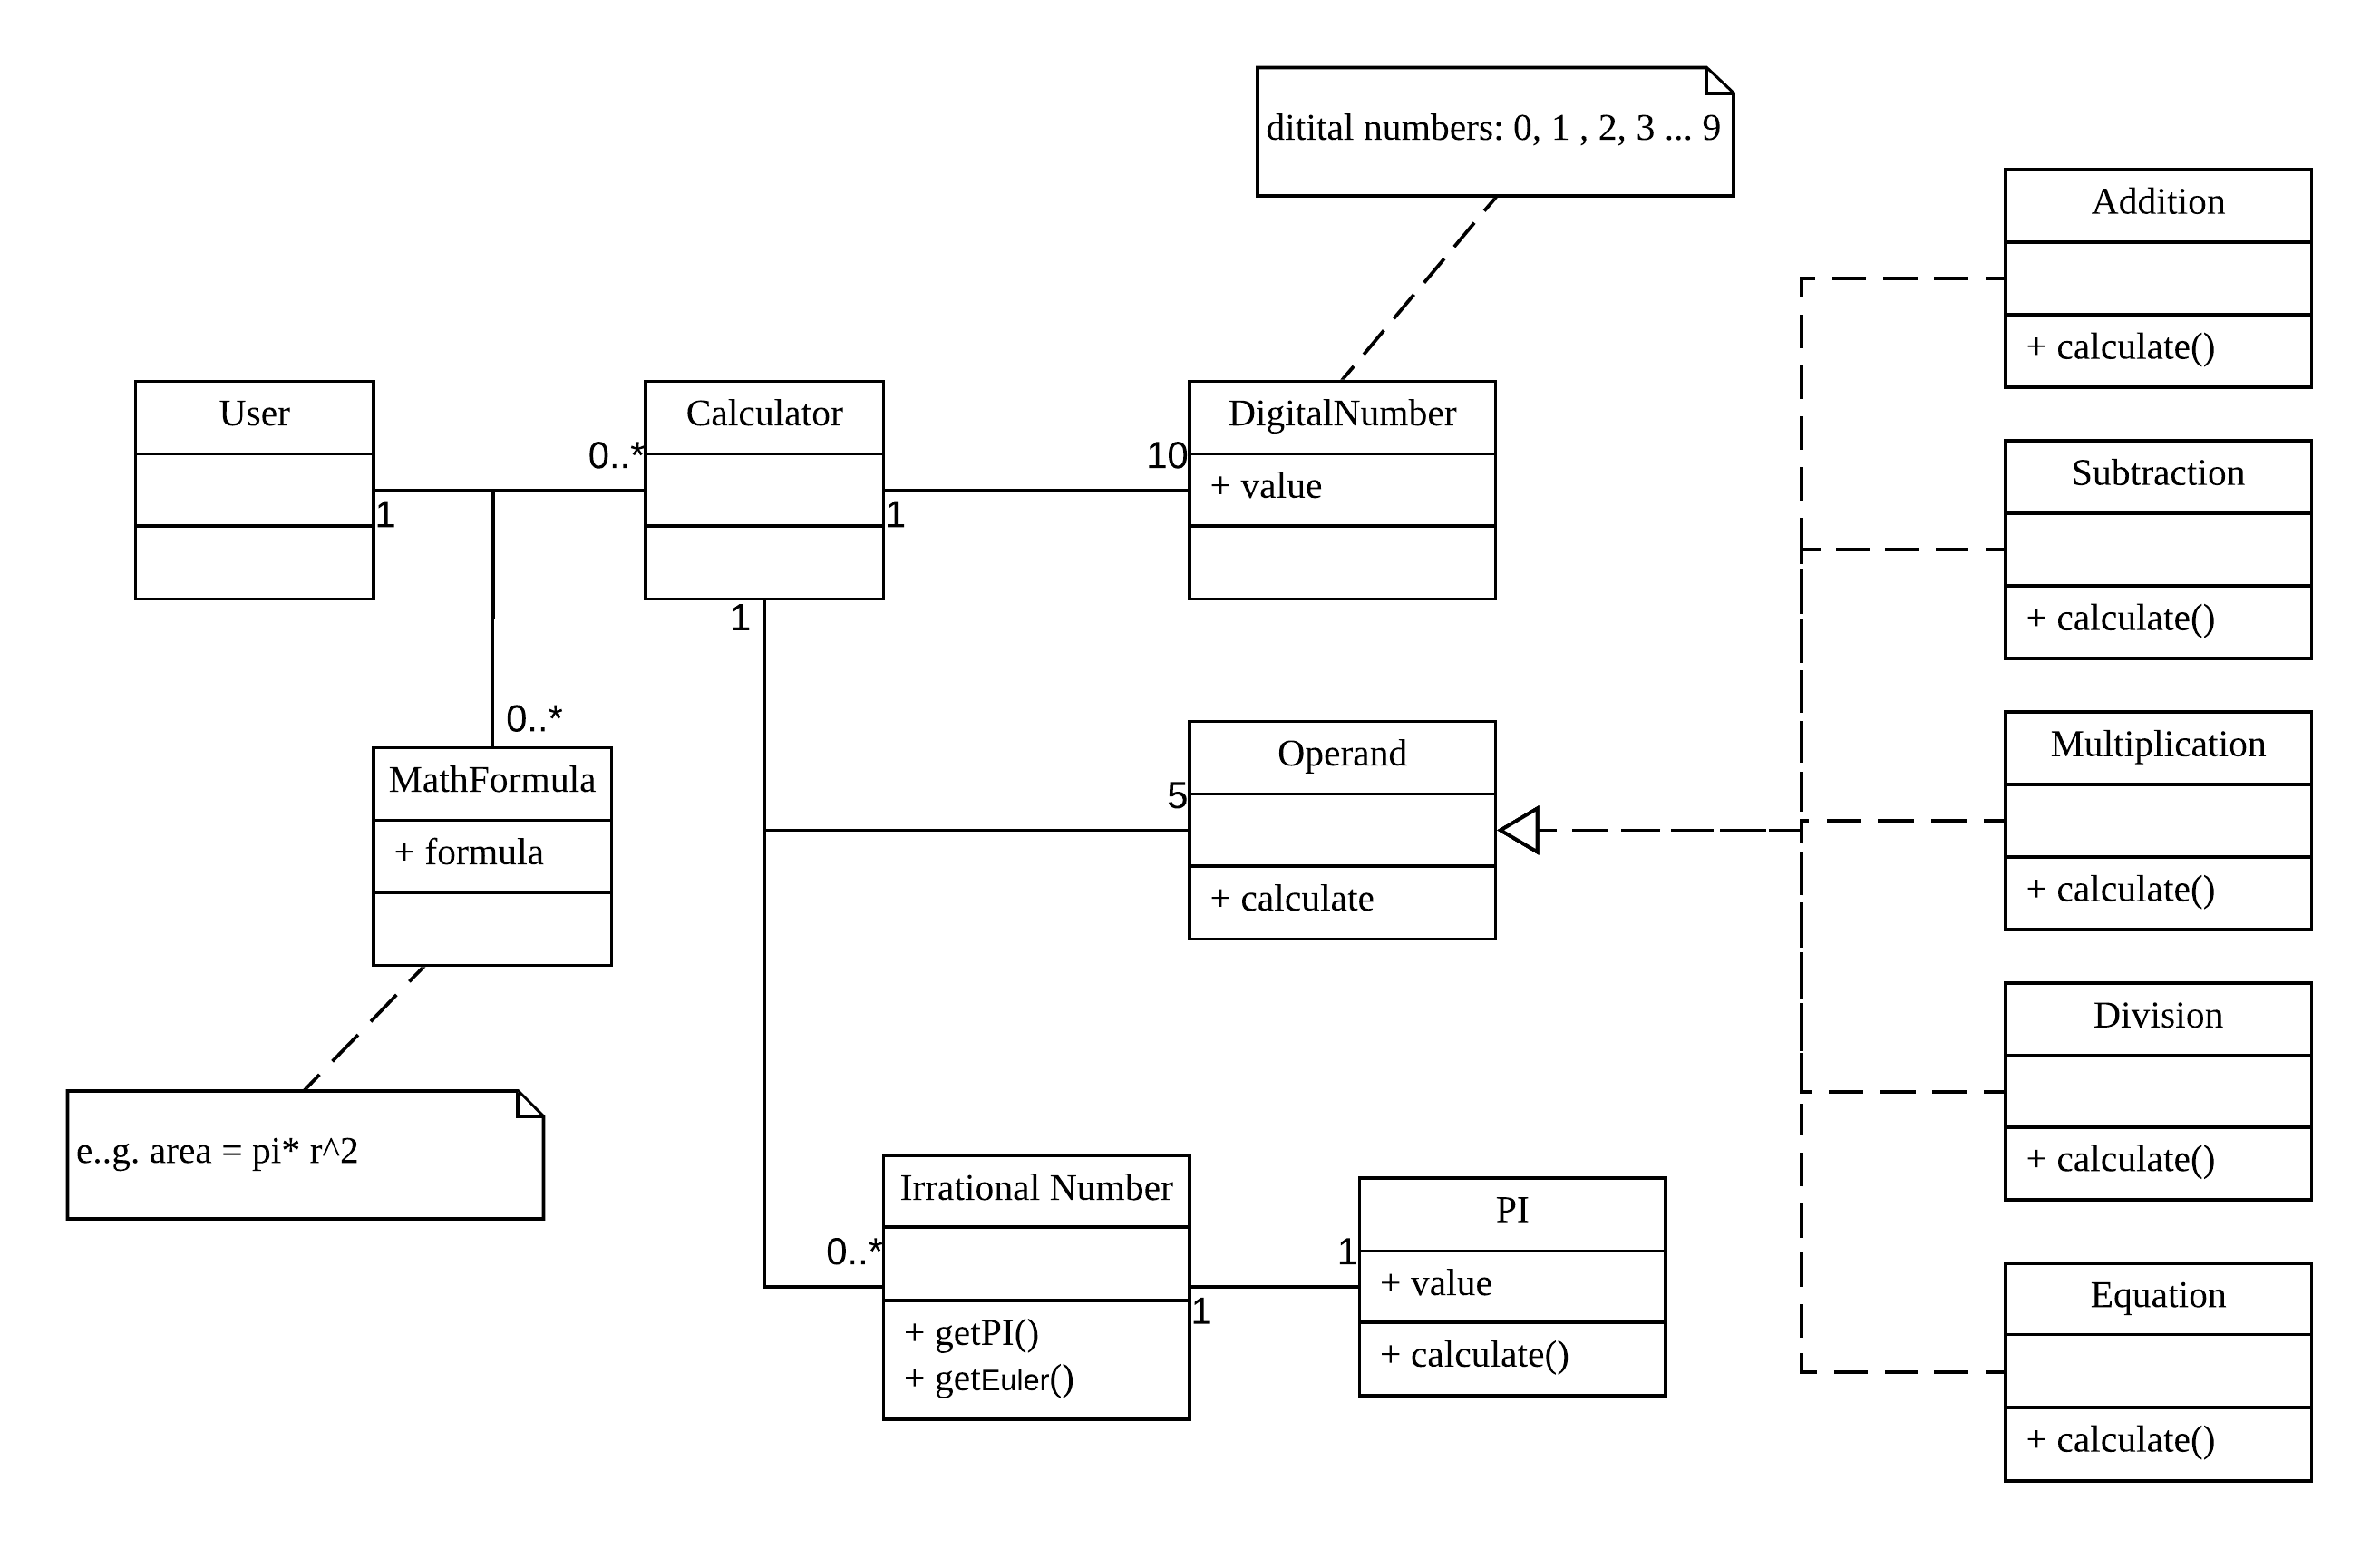
\includegraphics[width=\textwidth]{assets/Domain_Model.png}
		\caption{Domain Model}
		\label{fig:universe}
	\end{figure}
	
	
Each of the calculators has 10 digital numbers (from 0 to 9), 5 operands (+-*/=) and the irrational numbers (in this project is PI). 5 different operands can be responsible for a different task. For example, addition is one of the operands which responsible for adding the value, subtraction is also one of the operands which responsible for subtracting the value etc. In addition, an irrational number is a set of irrational numbers that might be used in a formula. User can solve a formula with Calculator. 

\chapter{Use Case Models} 

\begin{figure}[h!]
\section{Activity Diagram}
The calculator is started by showing a 0 value on the screen, then users can input the digital numbers or pi as one of the variables in the formula, then select an operand(/*-+=), if selected operand is not "=", then it means the calculation is not finished, save the previous value and  go back to let user select other numbers, until user choose "=" as the operand which means the formula is finished, its time to show the result. And the user can always press the clear button to clear the result and start from the beginning.

		\centering{
		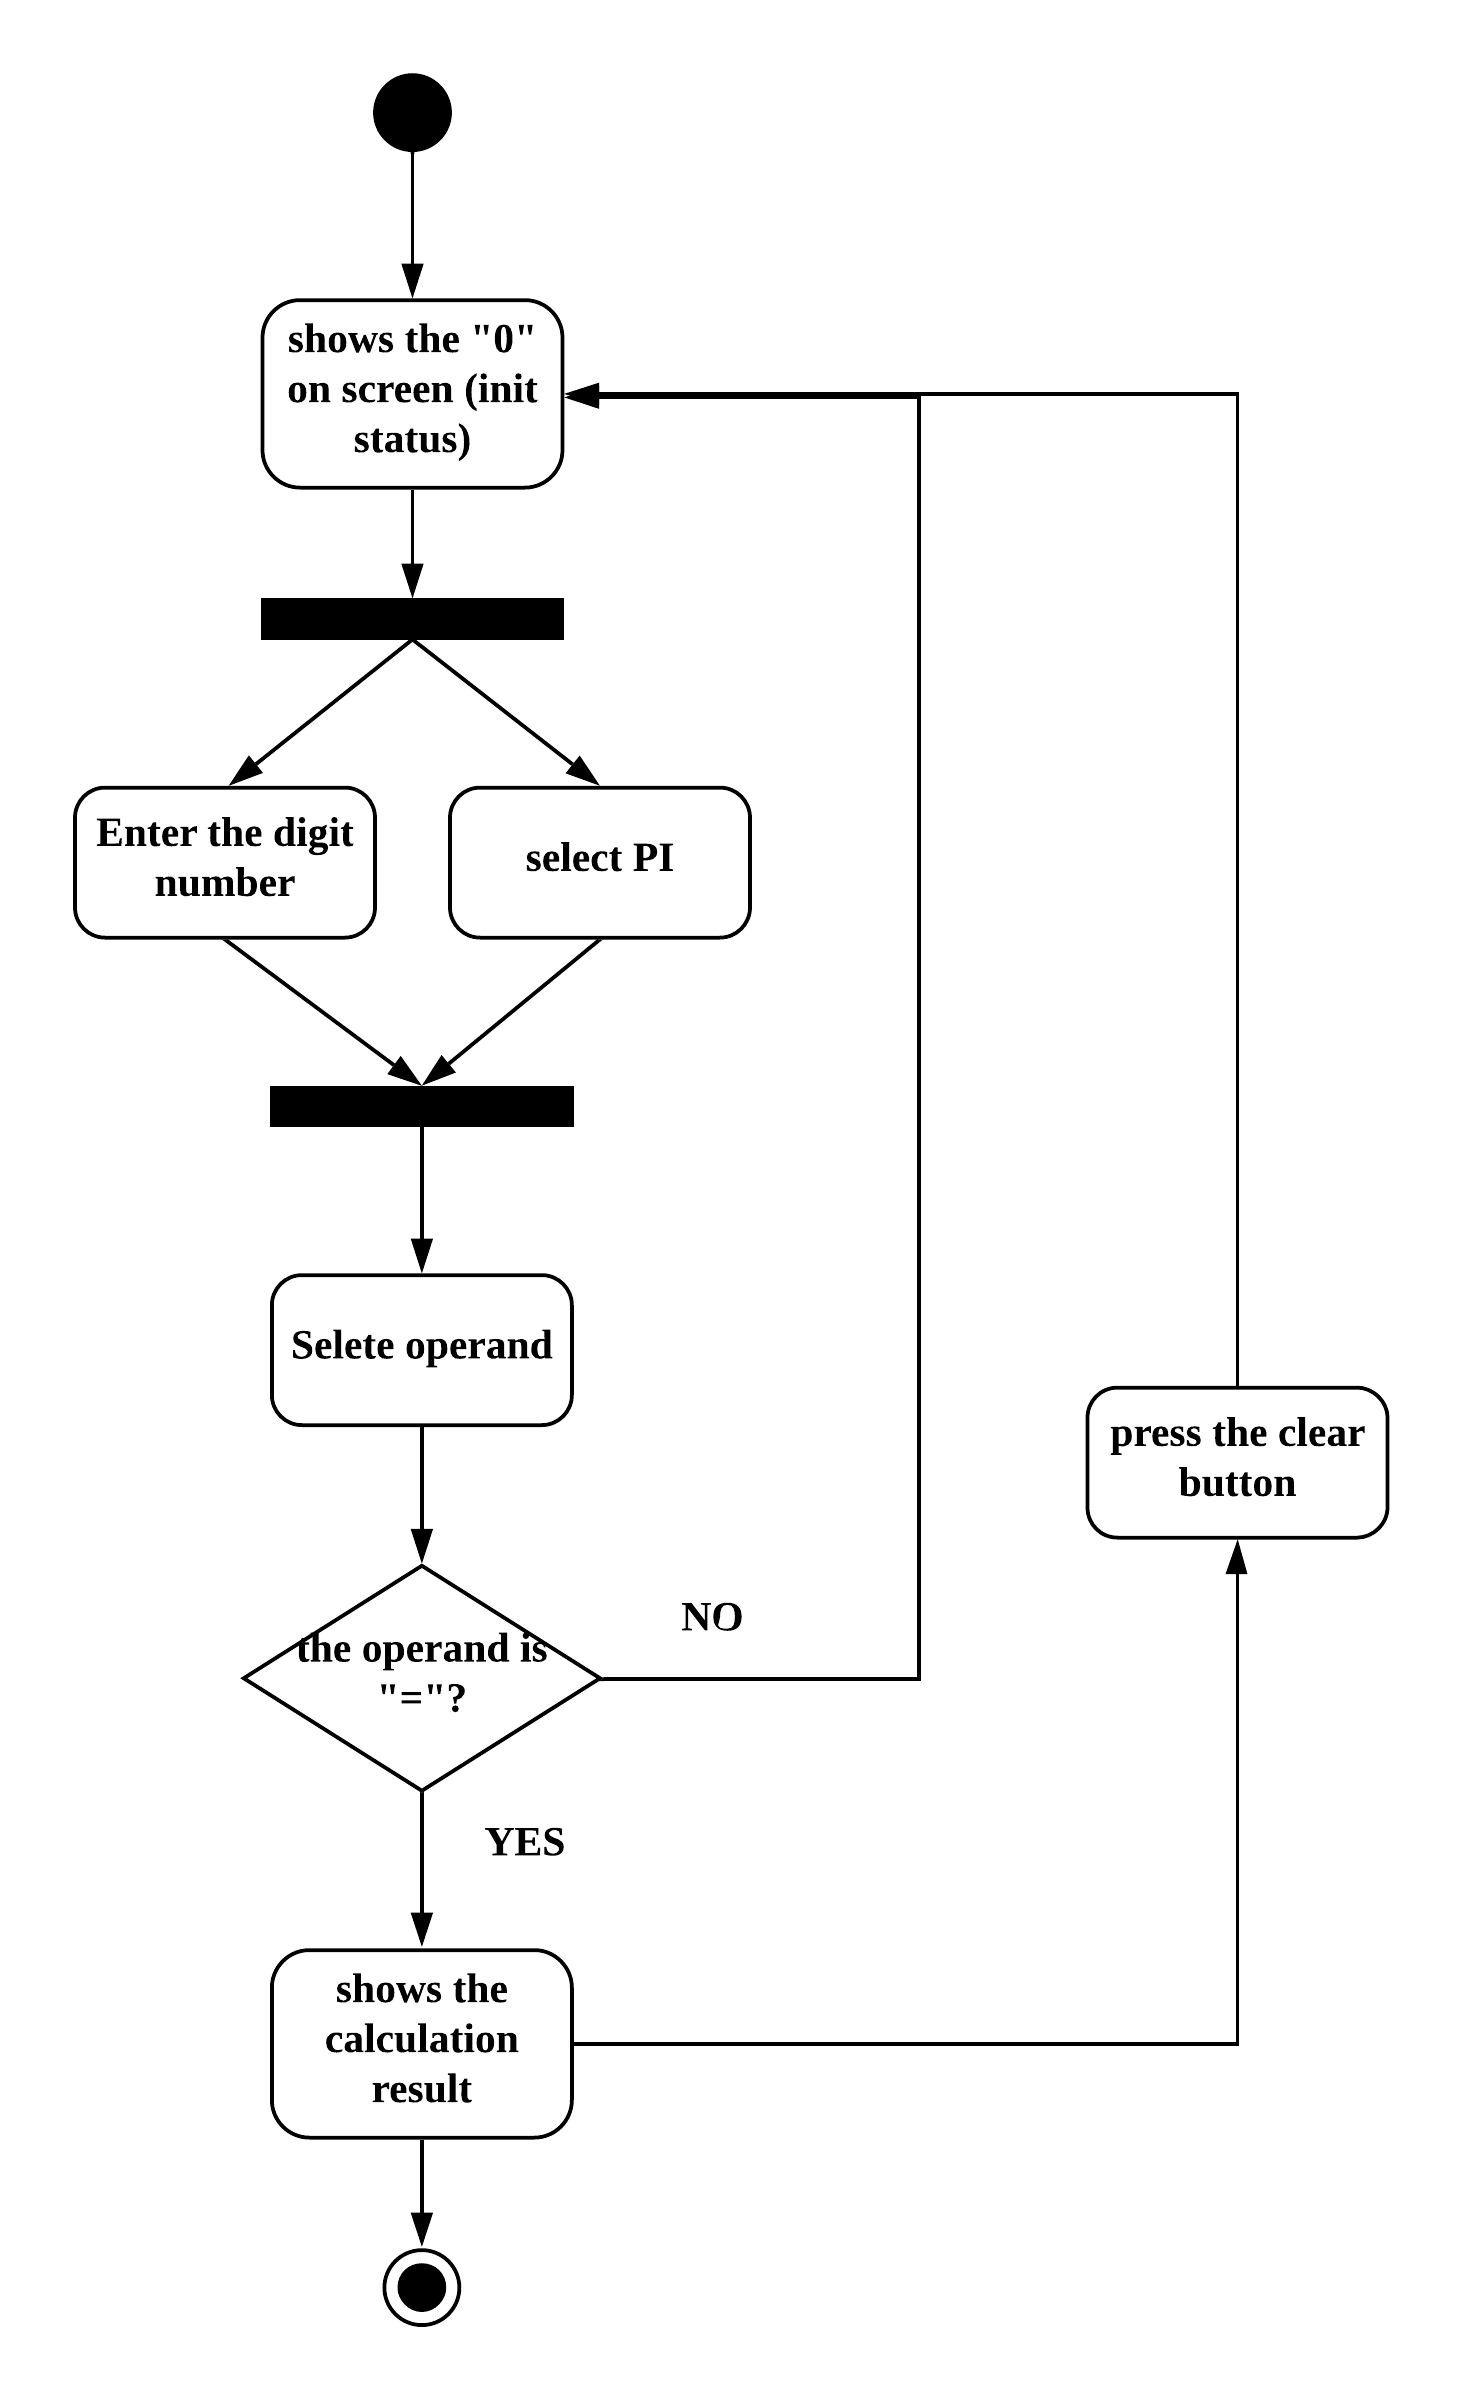
\includegraphics[scale=0.8]{assets/Activity_Diagram.png}
		\caption{Activity Diagram}
		\label{fig:universe} 
		}
	\end{figure}
	

	


	\begin{figure}[h!]
	\section{Use Case Diagram}
	
	\begin{itemize}
	The role is for the problem domain is user, he or she can clear the result, calculate the result, choose the operand, enter the digital numbers, user irrational numbers like Pi or calculate the area of the circle which is a function that will automatically apply an area calculation formula in the calculator.

  \item Clear the result: Clear the result on the screen, and clear all previous calculations. 
  \item Calculate the result:  Get the final result of the one-time calculation and show it on the screen. 
  \item Choose the operand: User can choose an operand from /*-+=, and it will be saved as the part of the calculation.
  \item Enter the digital numbers: user can choose a digital number from 0 to 9 and it will be saved as one of the variables in that calculation.

  \item Use irrational numbers: user can choose the irrational numbers such as pi in this case, as a part of the calculation.
  \item Use number pi: it is one of the options for irrational numbers, it will calculate the pi and return pi to the user.
  
  \item calculate the area of the circle: this is a special use case for my calculator, which has a function to directly perform a formula using pi to calculate the area of the circle.
  
\end{itemize}

	
		\centering{
			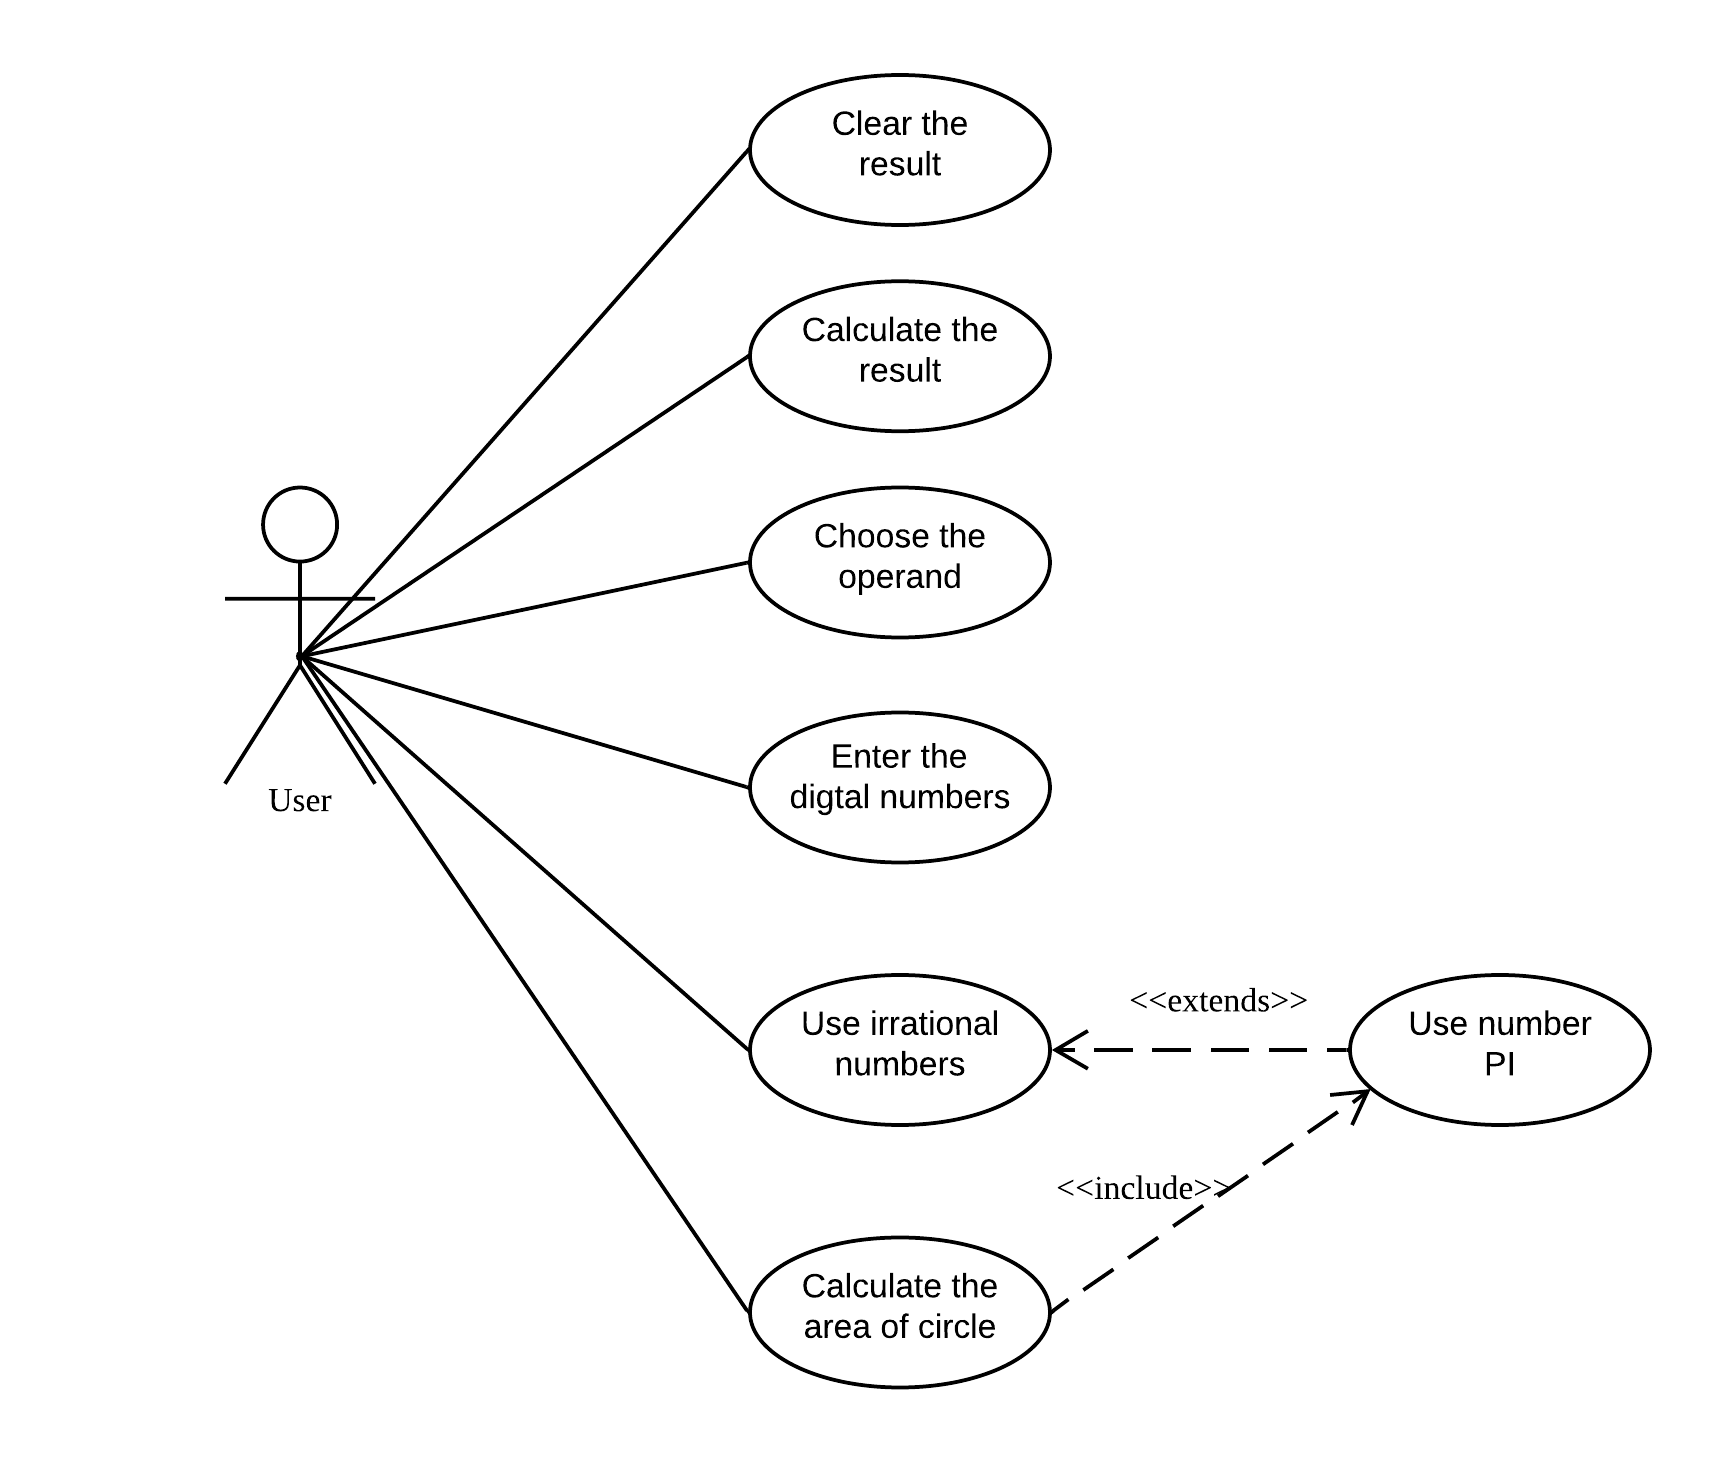
\includegraphics[width=\textwidth]{assets/Use_Case_Diagram.png}
		\caption{Use Case Diagram}
		\label{fig:universe}
		}
	
	\end{figure}
	












%-------------------------------------------------------------------------------
% REFERENCES
%-------------------------------------------------------------------------------
\newpage
	\bibliographystyle{plain}
	\bibliography{assets/references}

%[2]John W. Eaton, David Bateman, Sren Hauberg, Rik Wehbring (2015). GNU
%Octave version 4.0.0 manual: a high-level interactive language for numer-
%ical computations. Available: http://www.gnu.org/software/octave/doc/
%interpreter/. 
}
\end{document}

%-------------------------------------------------------------------------------
% SNIPPETS
%-------------------------------------------------------------------------------

%\begin{figure}[!ht]
%	\centering
%	\includegraphics[width=0.8\textwidth]{file_name}
%	\caption{}
%	\centering
%	\label{label:file_name}
%\end{figure}

%\begin{figure}[!ht]
%	\centering
%	\includegraphics[width=0.8\textwidth]{graph}
%	\caption{Blood pressure ranges and associated level of hypertension (American Heart Association, 2013).}
%	\centering
%	\label{label:graph}
%\end{figure}

%\begin{wrapfigure}{r}{0.30\textwidth}
%	\vspace{-40pt}
%	\begin{center}
%		\includegraphics[width=0.29\textwidth]{file_name}
%	\end{center}
%	\vspace{-20pt}
%	\caption{}
%	\label{label:file_name}
%\end{wrapfigure}

%\begin{wrapfigure}{r}{0.45\textwidth}
%	\begin{center}
%		\includegraphics[width=0.29\textwidth]{manometer}
%	\end{center}
%	\caption{Aneroid sphygmomanometer with stethoscope (Medicalexpo, 2012).}
%	\label{label:manometer}
%\end{wrapfigure}

%\begin{table}[!ht]\footnotesize
%	\centering
%	\begin{tabular}{cccccc}
%	\toprule
%	\multicolumn{2}{c} {Pearson's correlation test} & \multicolumn{4}{c} {Independent t-test} \\
%	\midrule	
%	\multicolumn{2}{c} {Gender} & \multicolumn{2}{c} {Activity level} & \multicolumn{2}{c} {Gender} \\
%	\midrule
%	Males & Females & 1st level & 6th level & Males & Females \\
%	\midrule
%	\multicolumn{2}{c} {BMI vs. SP} & \multicolumn{2}{c} {Systolic pressure} & \multicolumn{2}{c} {Systolic Pressure} \\
%	\multicolumn{2}{c} {BMI vs. DP} & \multicolumn{2}{c} {Diastolic pressure} & \multicolumn{2}{c} {Diastolic pressure} \\
%	\multicolumn{2}{c} {BMI vs. MAP} & \multicolumn{2}{c} {MAP} & \multicolumn{2}{c} {MAP} \\
%	\multicolumn{2}{c} {W:H ratio vs. SP} & \multicolumn{2}{c} {BMI} & \multicolumn{2}{c} {BMI} \\
%	\multicolumn{2}{c} {W:H ratio vs. DP} & \multicolumn{2}{c} {W:H ratio} & \multicolumn{2}{c} {W:H ratio} \\
%	\multicolumn{2}{c} {W:H ratio vs. MAP} & \multicolumn{2}{c} {\% Body fat} & \multicolumn{2}{c} {\% Body fat} \\
%	\multicolumn{2}{c} {} & \multicolumn{2}{c} {Height} & \multicolumn{2}{c} {Height} \\
%	\multicolumn{2}{c} {} & \multicolumn{2}{c} {Weight} & \multicolumn{2}{c} {Weight} \\
%	\multicolumn{2}{c} {} & \multicolumn{2}{c} {Heart rate} & \multicolumn{2}{c} {Heart rate} \\
%	\bottomrule
%	\end{tabular}
%	\caption{Parameters that were analysed and related statistical test performed for current study. BMI - body mass index; SP - systolic pressure; DP - diastolic pressure; MAP - mean arterial pressure; W:H ratio - waist to hip ratio.}
%	\label{label:tests}
%\end{table}%\documentclass{article}
%\usepackage[utf8]{inputenc}

%\title{Weekly Report template}
%\author{gandhalijuvekar }
%\date{January 2019}

%\begin{document}

%\maketitle

%\section{Introduction}

%\end{document}
